% =====================================================================
% Modelagem do grafo --- Brunno (Frente 1)
% Só o Brunno edita este arquivo.
% =====================================================================
\section{Modelagem do grafo}\label{sec:modelagem}

Cada rede vira um grafo simples $G = (V, E)$, com $n = |V|$ nós e $m = |E|$ arestas. Na Twitch PT,
cada nó é um streamer e cada aresta, uma amizade mútua, sem peso; na Network of Thrones, o peso
$w(e)$ é o número de interações entre os dois personagens; nas redes sem peso, $w(e) = 1$.

\paragraph{Estrutura.} As redes sociais são esparsas: na Twitch PT, só 1,7\% dos pares possíveis
são amizades. Uma matriz de adjacência guardaria $n^2 = 3{,}66$ milhões de células, 98\% delas com
zero, e a busca em largura, base de quase todos os algoritmos do trabalho, custaria $\Theta(n^2)$; a
lista de adjacência guarda só as arestas que existem, em $O(n + m)$, e faz a mesma busca em
$\Theta(n + m)$~\cite{cormen2022}. A classe \codigo{Grafo} guarda essa lista como um dicionário de
dicionários, em que \codigo{\_adj[v][w]} é o peso da aresta entre $v$ e $w$. Assim, inserir um nó,
inserir ou remover uma aresta, testar se ela existe e ler o peso e o grau custam $O(1)$ em
média~\cite{pythoncomplexidade}; percorrer os vizinhos de $v$ custa $O(\text{grau}(v))$, e contar os
nós e as arestas, $O(1)$, porque $m$ é atualizado a cada inserção e remoção. O peso fica junto do
vizinho, o que atende a Network of Thrones e o Louvain, que cria arestas com peso ao agrupar
comunidades, e os nós podem ser de qualquer tipo imutável, como números na Twitch PT e nomes na
Network of Thrones. O NetworkX adota a mesma estrutura pelos mesmos motivos~\cite{hagberg2008}.

\paragraph{Outras decisões.} No grafo direcionado, a classe guarda à parte os predecessores de cada
nó (\codigo{\_pred}), para o grau de entrada e o PageRank~\cite{brin1998}; no não direcionado,
\codigo{\_pred} é o próprio \codigo{\_adj}, sem cópia. Os laços, que o Louvain cria ao agrupar
comunidades, contam duas vezes no grau, para a soma dos graus ser sempre $2m$. Nos algoritmos mais
pesados, o \codigo{IndexadorDeNos} renumera os nós de $0$ a $n-1$, e a adjacência vira uma lista de
listas, que o Python percorre mais depressa que dicionários.

\paragraph{Diagramas.} A Figura~\ref{fig:uml} mostra o núcleo e os pacotes. Os demais pacotes são
módulos de funções que recebem um \codigo{Grafo}, não o alteram e devolvem um valor por nó
(\codigo{dict[nó, valor]}), um contrato comum a todo o grupo; os leitores e os geradores criam
grafos, a interface só chama as funções, e o NetworkX aparece apenas em \codigo{desempenho/}. A
Figura~\ref{fig:uml-comportamento} traz os diagramas comportamentais da Etapa 1, que estão em tamanho
real em \codigo{documentos/uml/}.

\begin{figure}[htbp]
\centering
\begin{minipage}[b]{.52\textwidth}
  \centering
  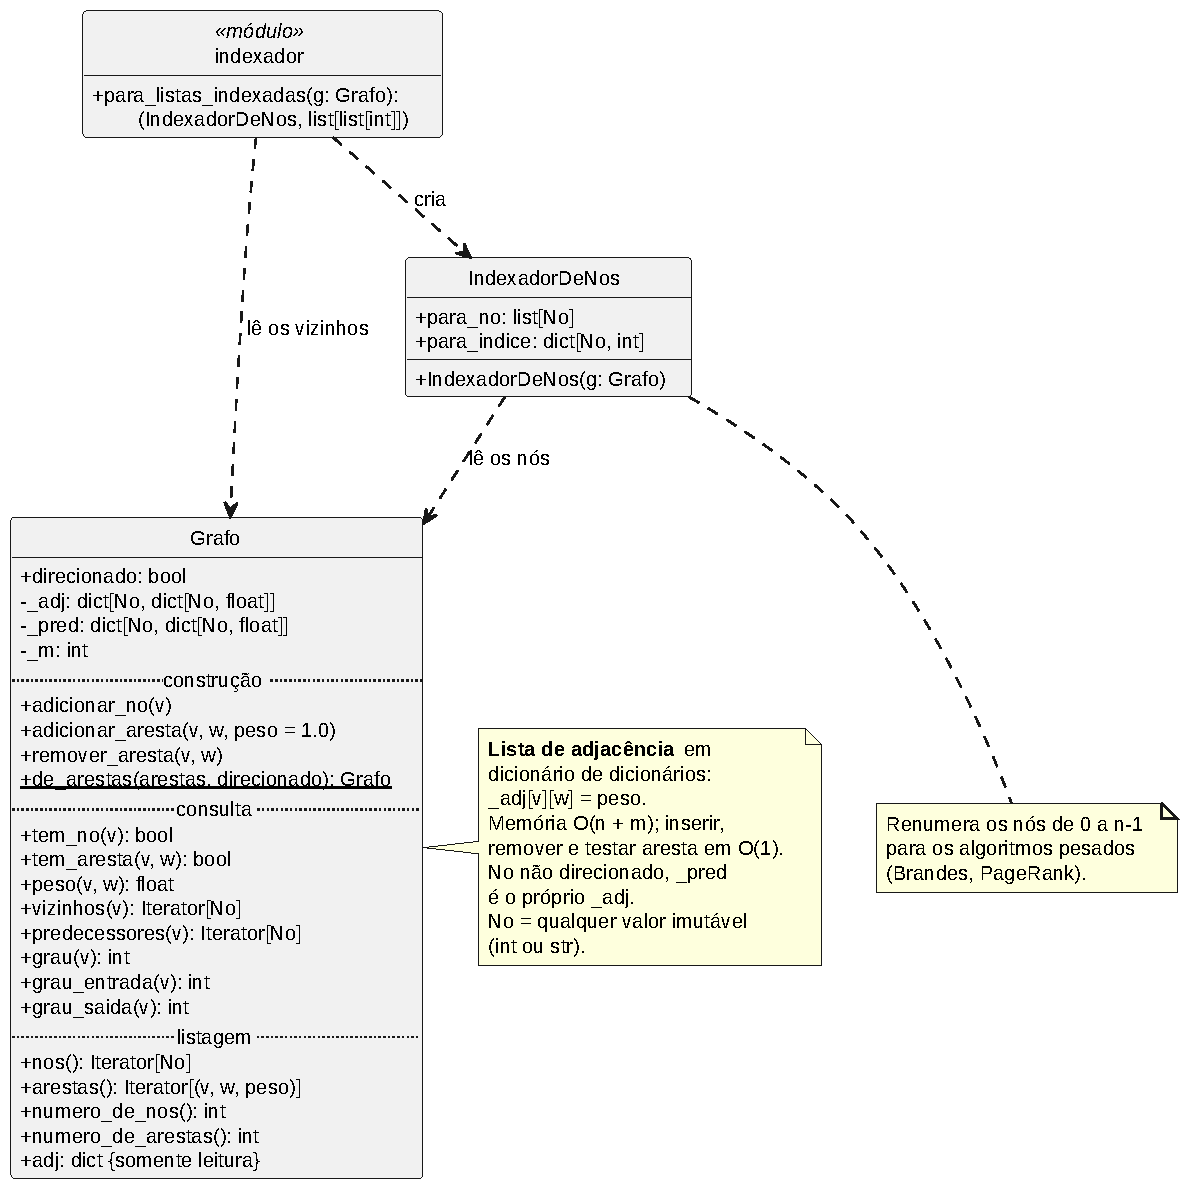
\includegraphics[width=\textwidth]{classes.pdf}\\[2pt]
  {\small (a) Classes do núcleo (\codigo{redes/nucleo})}
\end{minipage}\hfill
\begin{minipage}[b]{.36\textwidth}
  \centering
  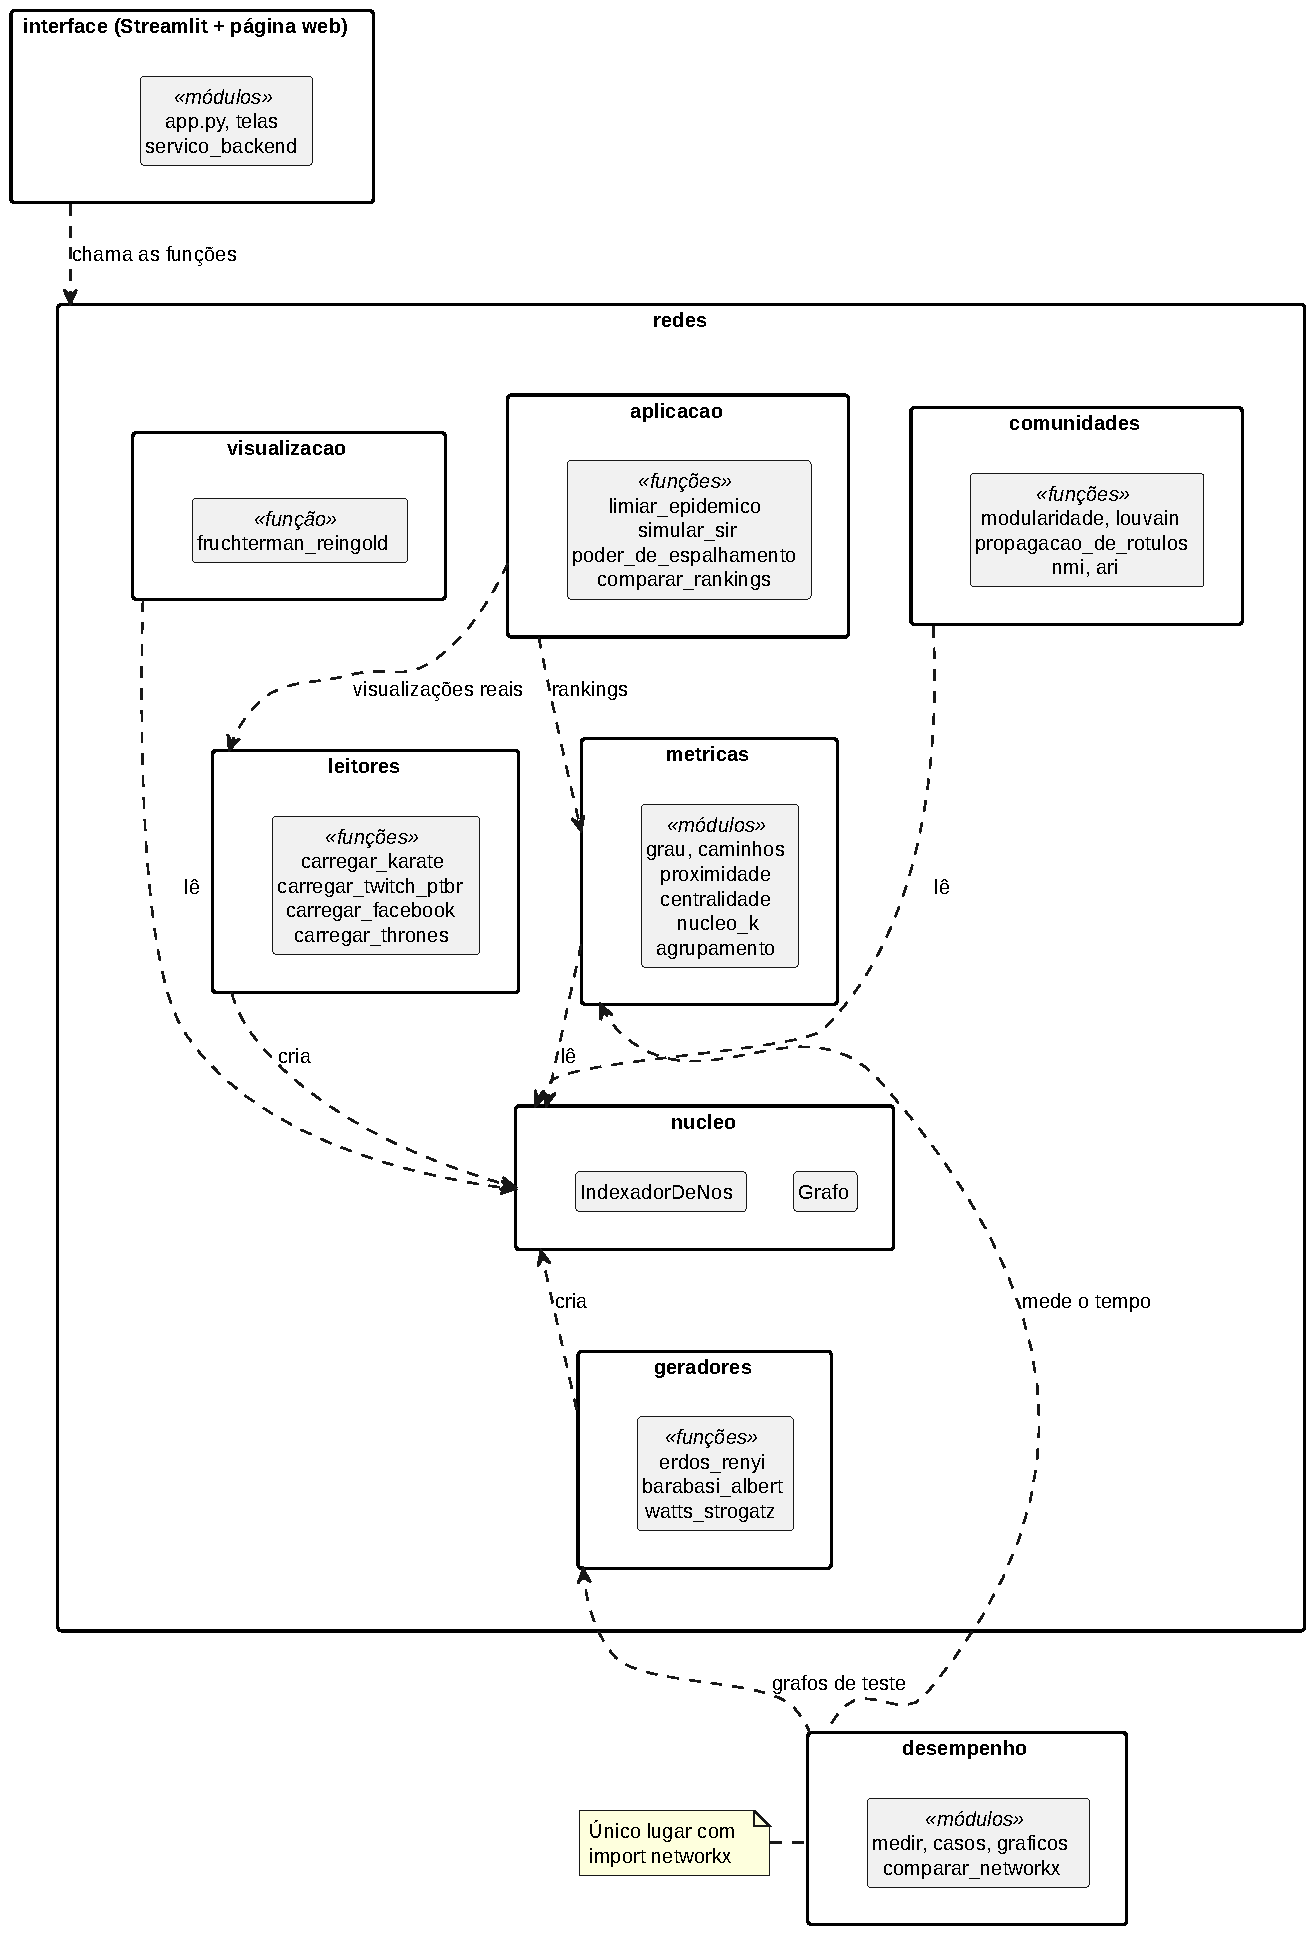
\includegraphics[width=\textwidth]{pacotes.pdf}\\[2pt]
  {\small (b) Pacotes}
\end{minipage}
\caption{Diagramas UML da estrutura do código. Em (b), as setas tracejadas indicam dependência:
quem aponta usa o pacote apontado.}
\label{fig:uml}
\end{figure}

\begin{figure}[htbp]
\centering
\begin{minipage}[b]{.38\textwidth}
  \centering
  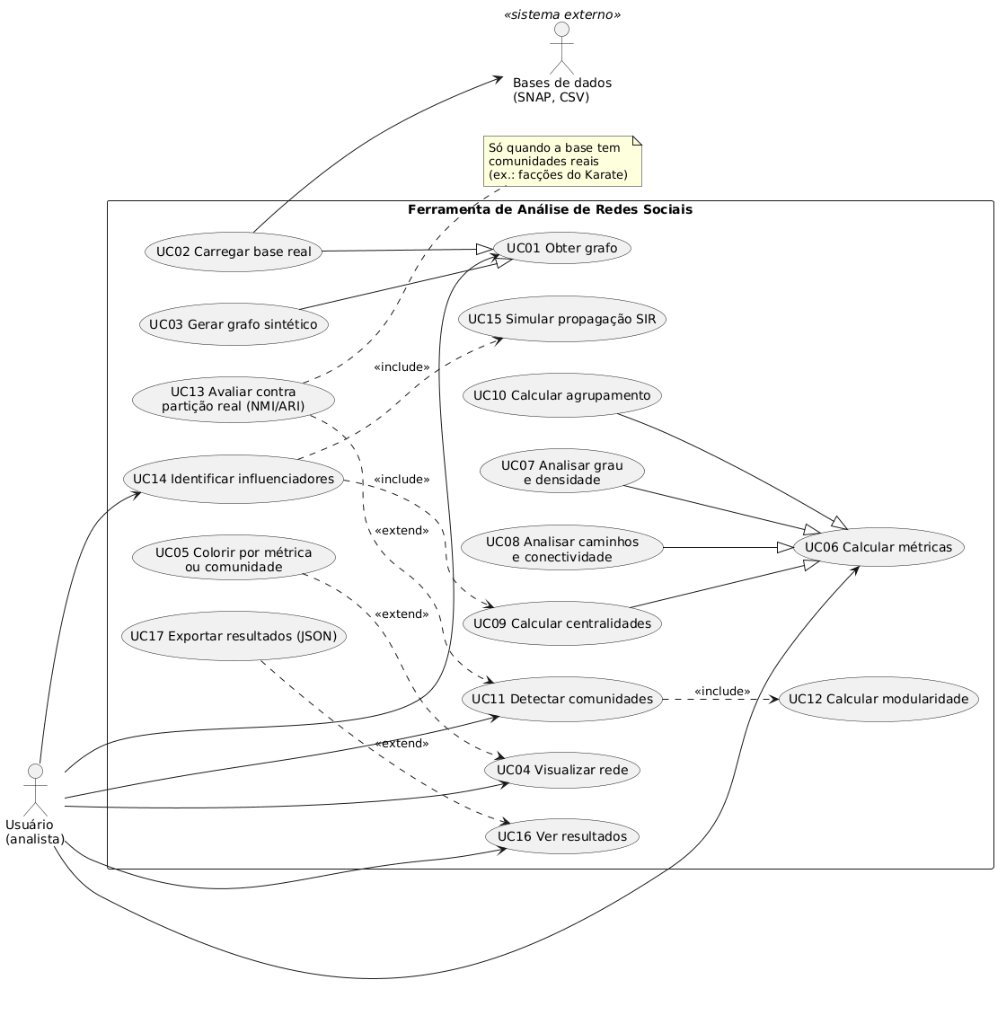
\includegraphics[width=\textwidth]{casos_de_uso.jpg}\\[2pt]
  {\small (a) Casos de uso}
\end{minipage}\hfill
\begin{minipage}[b]{.33\textwidth}
  \centering
  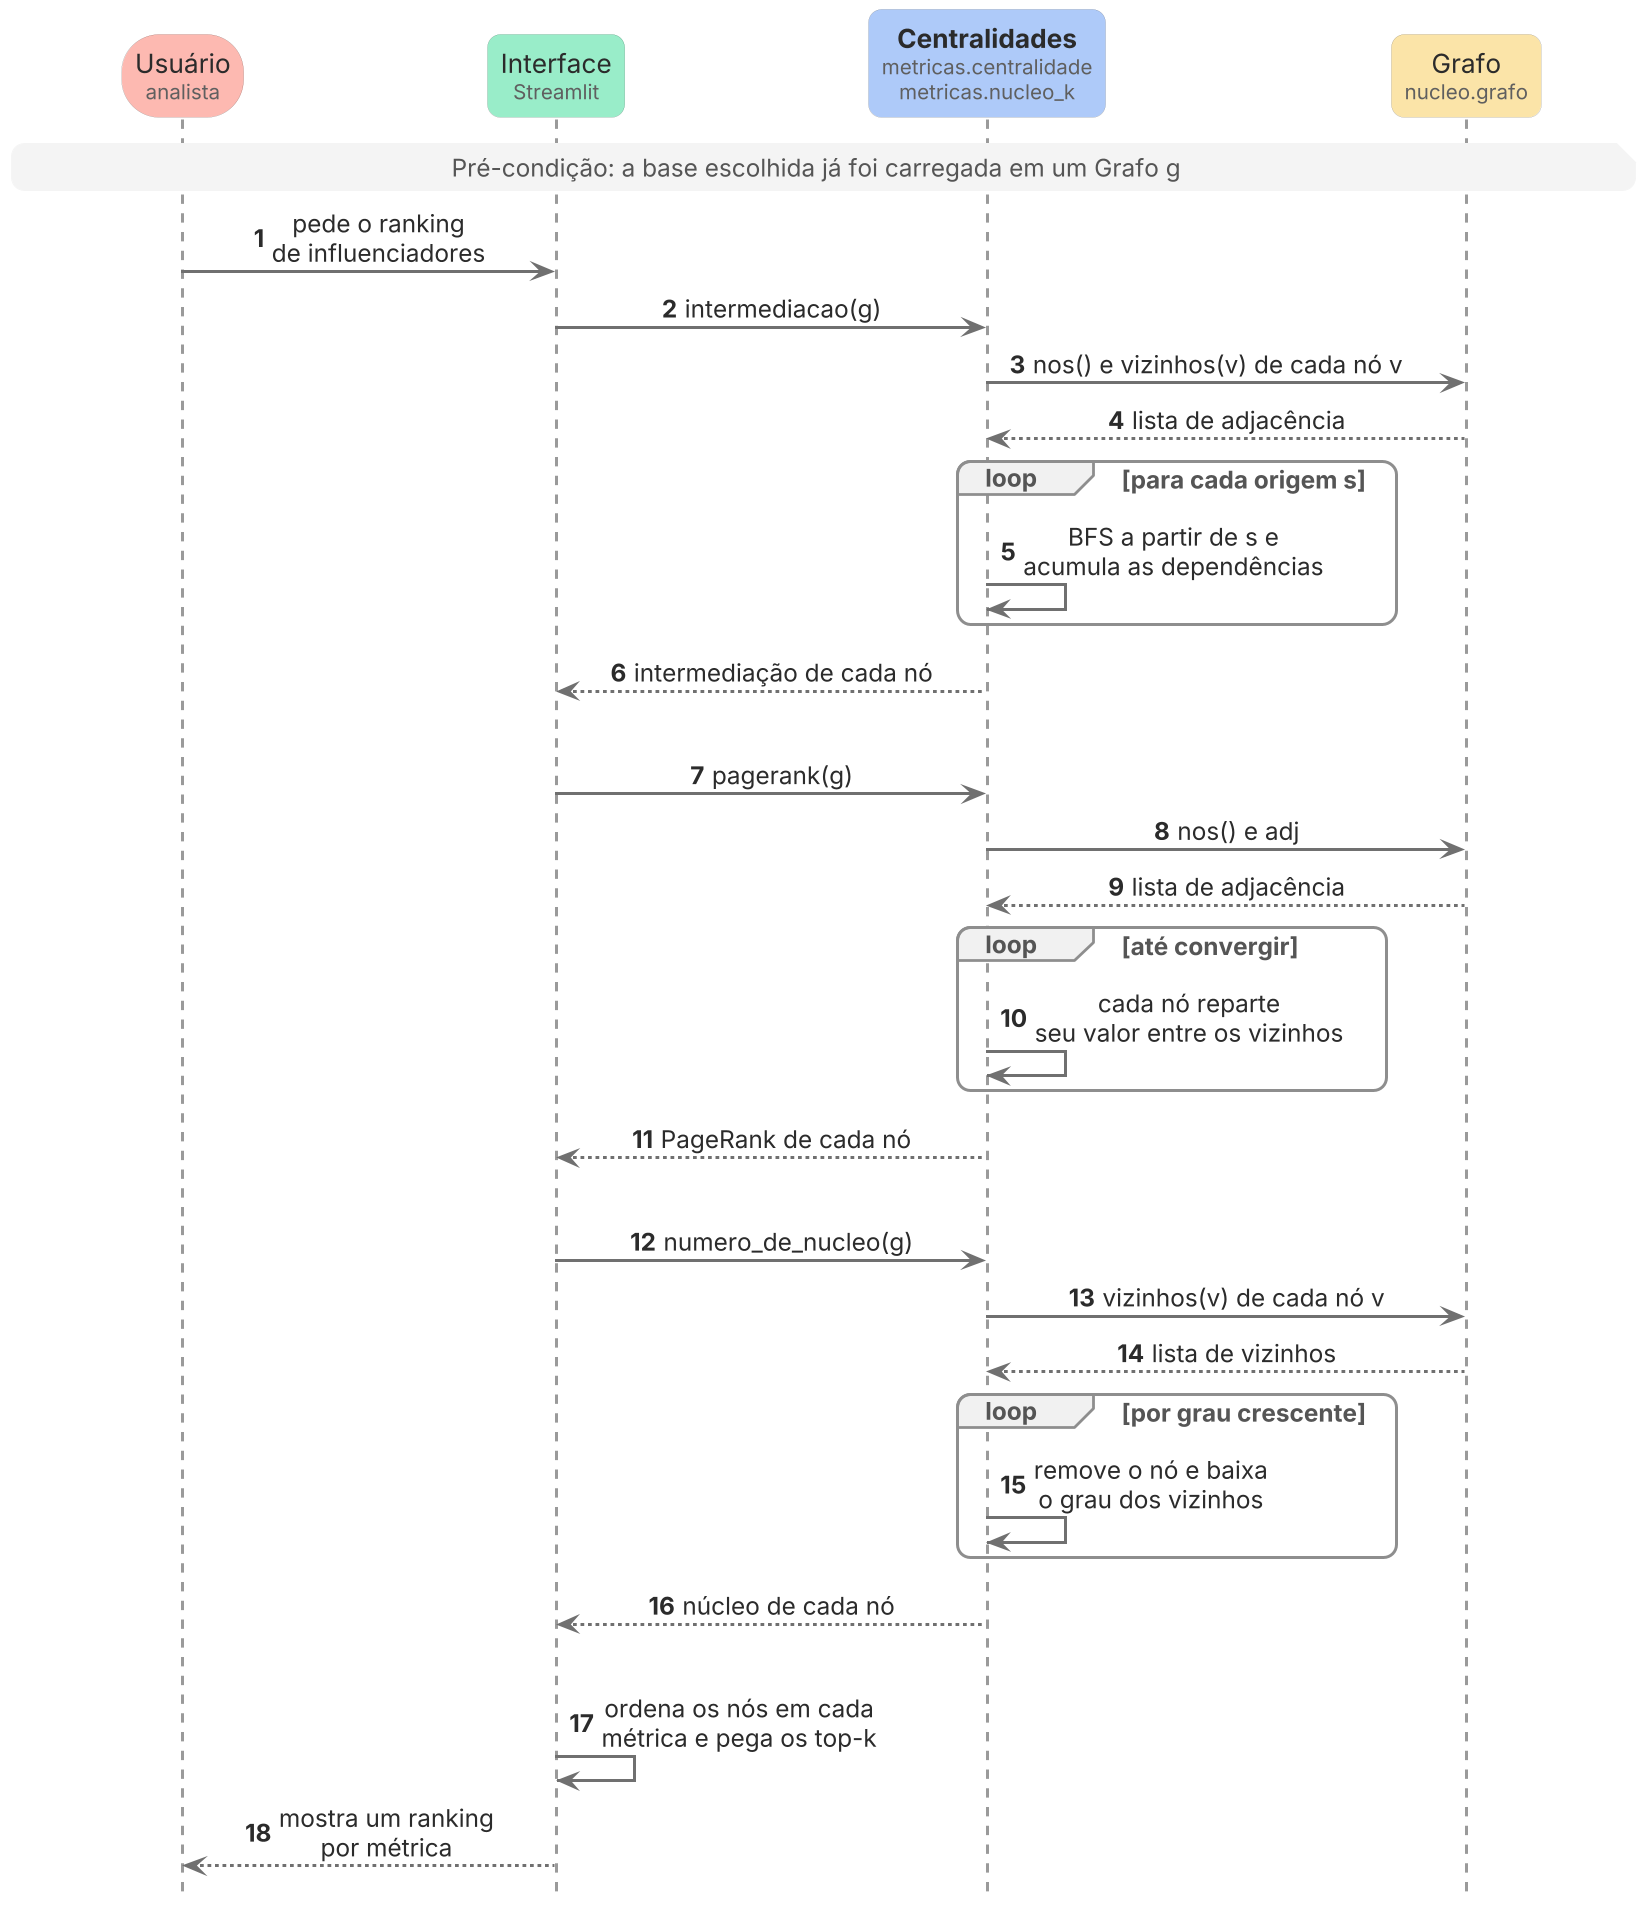
\includegraphics[width=\textwidth]{sequencia.png}\\[2pt]
  {\small (b) Sequência do ranking}
\end{minipage}\hfill
\begin{minipage}[b]{.21\textwidth}
  \centering
  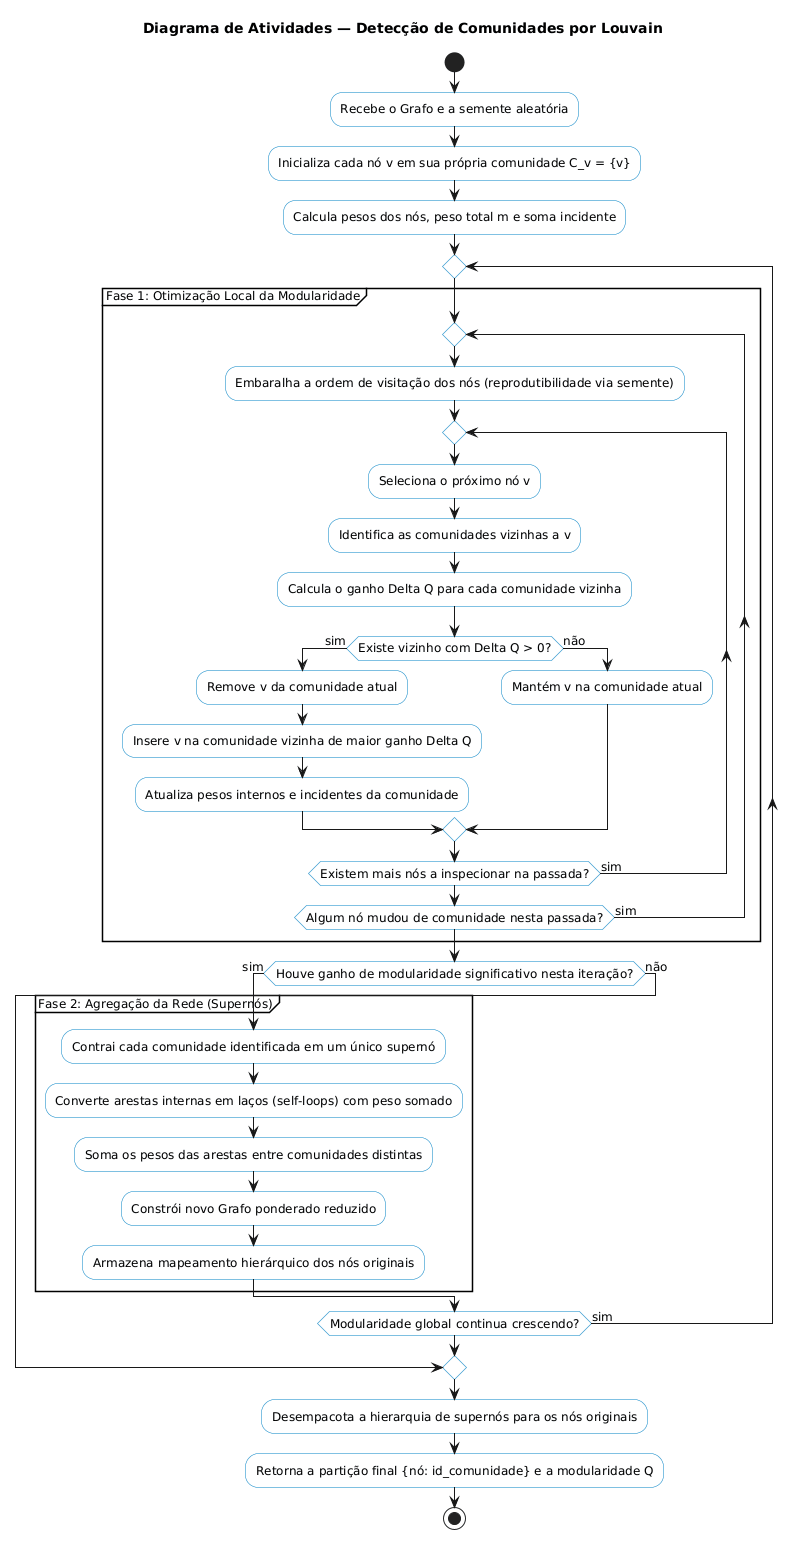
\includegraphics[width=\textwidth]{atividades_louvain.png}\\[2pt]
  {\small (c) Atividades do Louvain}
\end{minipage}
\caption{Diagramas comportamentais da Etapa 1: (a) os 17 casos de uso da ferramenta; (b) as chamadas
que montam o ranking de influenciadores; (c) as duas fases do método de Louvain.}
\label{fig:uml-comportamento}
\end{figure}

\paragraph{Corretude.} A classe, os leitores e os geradores têm 41 testes (\codigo{pytest}): grafos
de resposta conhecida, como o completo $K_5$; propriedades conferidas pelo \codigo{Hypothesis} em
centenas de grafos aleatórios, como a soma dos graus ser $2m$; os tamanhos das quatro bases; e o
número de arestas de cada gerador.
